\section{Resultados Computacionais}

\subsection{Planejamento e validação dos experimentos}

Esta revisão reexecutou os três problemas em cinco sementes ($42$, $123$, $456$, $789$, $1011$), totalizando 15 buscas. Os parâmetros da Tabela~\ref{tab:parametros} e os pesos históricos de penalidade foram preservados. O retorno passou a ser a melhor solução viável observada, independentemente da incumbente por fitness.

Cada rodada tem composição, três objetivos, violações, status, histórico, contadores, motivo de parada e tempo decorrido em JSON. A releitura recalcula os valores; uma segunda rotina confere massa, compatibilidade, usos globais, faixas químicas e objetivos por contagens de minérios. As 15 soluções finais passaram pelas duas verificações. As estatísticas usam desvio-padrão amostral com denominador $n-1$.

\begin{table}[H]\centering\small

\caption{Resultados finais viáveis das cinco execuções por objetivo. Cada coluna corresponde a um problema otimizado separadamente.}

\label{tab:resultados}

\begin{tabular}{lrrr}\toprule

Execução & $f_1$ (R\$) & $f_2$ (p.p.$^2$) & $f_3$ (p.p.$^2$) \\ \midrule

1 (seed 42) & \num{60680000} & \num{2.373029} & \num{1.453254} \\

2 (seed 123) & \num{60400000} & \num{2.373828} & \num{1.450865} \\

3 (seed 456) & \num{60660000} & \num{2.372757} & \num{1.452078} \\

4 (seed 789) & \num{60300000} & \num{2.373927} & \num{1.436169} \\

5 (seed 1011) & \num{60480000} & \num{2.373844} & \num{1.443334} \\

\midrule

Mínimo & \num{60300000} & \num{2.372757} & \num{1.436169} \\

Média & \num{60504000} & \num{2.373477} & \num{1.447140} \\

Desvio-padrão & \num{164560} & \num{0.000543} & \num{0.007254} \\

Máximo & \num{60680000} & \num{2.373927} & \num{1.453254} \\

\bottomrule\end{tabular}\end{table}

\subsection{Esforço e parada}

Os tempos abaixo são de relógio e dependem da máquina e da instrumentação. Não são tempos de CPU nem devem ser comparados diretamente aos do log antigo.

\begin{table}[H]\centering\small

\caption{Esforço da campanha corrigida por objetivo}

\begin{tabular}{lrrrr}\toprule

Objetivo & Tempo médio (s) & Avaliações médias & Máx. iterações & Estagnação \\ \midrule

$f_1$ & \num{47.9} & \num{49434} & 4 & 1 \\

$f_2$ & \num{60.5} & \num{53562} & 2 & 3 \\

$f_3$ & \num{74.0} & \num{69886} & 5 & 0 \\

\bottomrule\end{tabular}\end{table}

\subsection{Curvas de convergência}

Cada figura sobrepõe as cinco sementes. O eixo vertical representa a melhor solução viável já observada, não o objetivo bruto da trajetória penalizada. Antes do primeiro candidato viável o valor é ausente; após esse momento, a curva não aumenta. A construtiva ($f_1=60{.}400{.}000$ R\$, $f_2\approx23{,}481055$, $f_3\approx14{,}909888$) tem 12 violações químicas e é apenas ponto de partida.

\begin{figure}[H]\centering

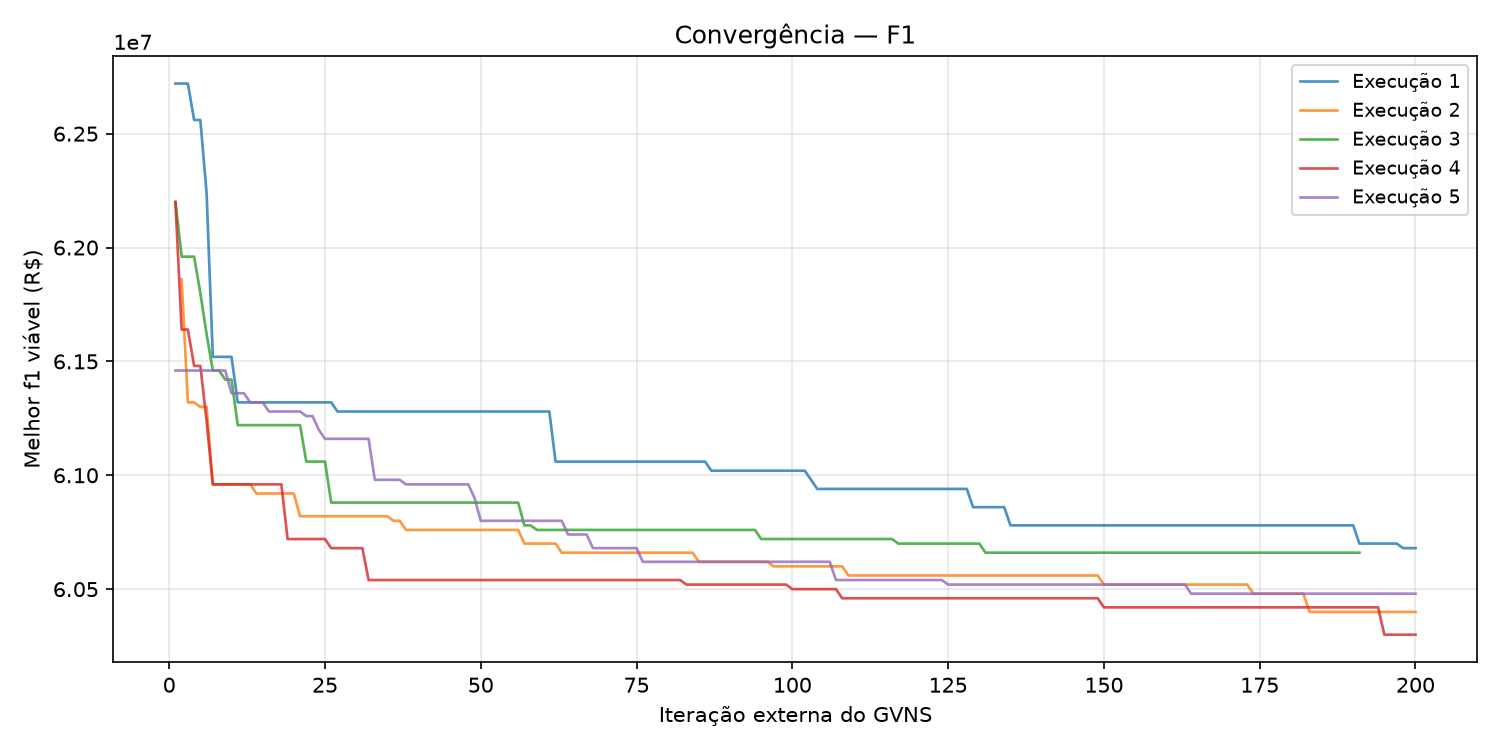
\includegraphics[width=0.88\textwidth]{results/tp1_corrigido/convergencia_f1.png}

\caption{Melhor valor viável observado de $f_1$ nas cinco execuções}

\label{fig:conv_f1}

\end{figure}

\begin{figure}[H]\centering

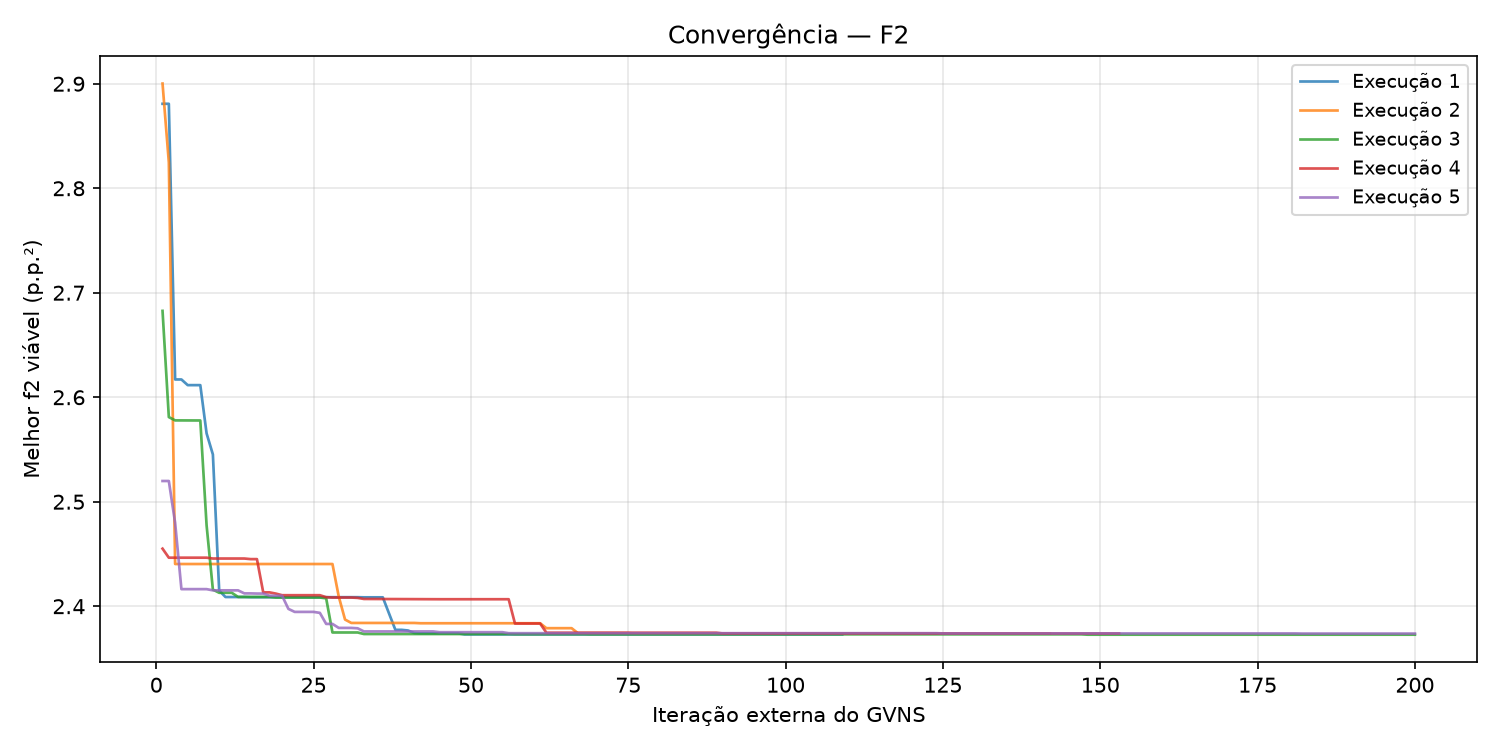
\includegraphics[width=0.88\textwidth]{results/tp1_corrigido/convergencia_f2.png}

\caption{Melhor valor viável observado de $f_2$ nas cinco execuções}

\label{fig:conv_f2}

\end{figure}

\begin{figure}[H]\centering

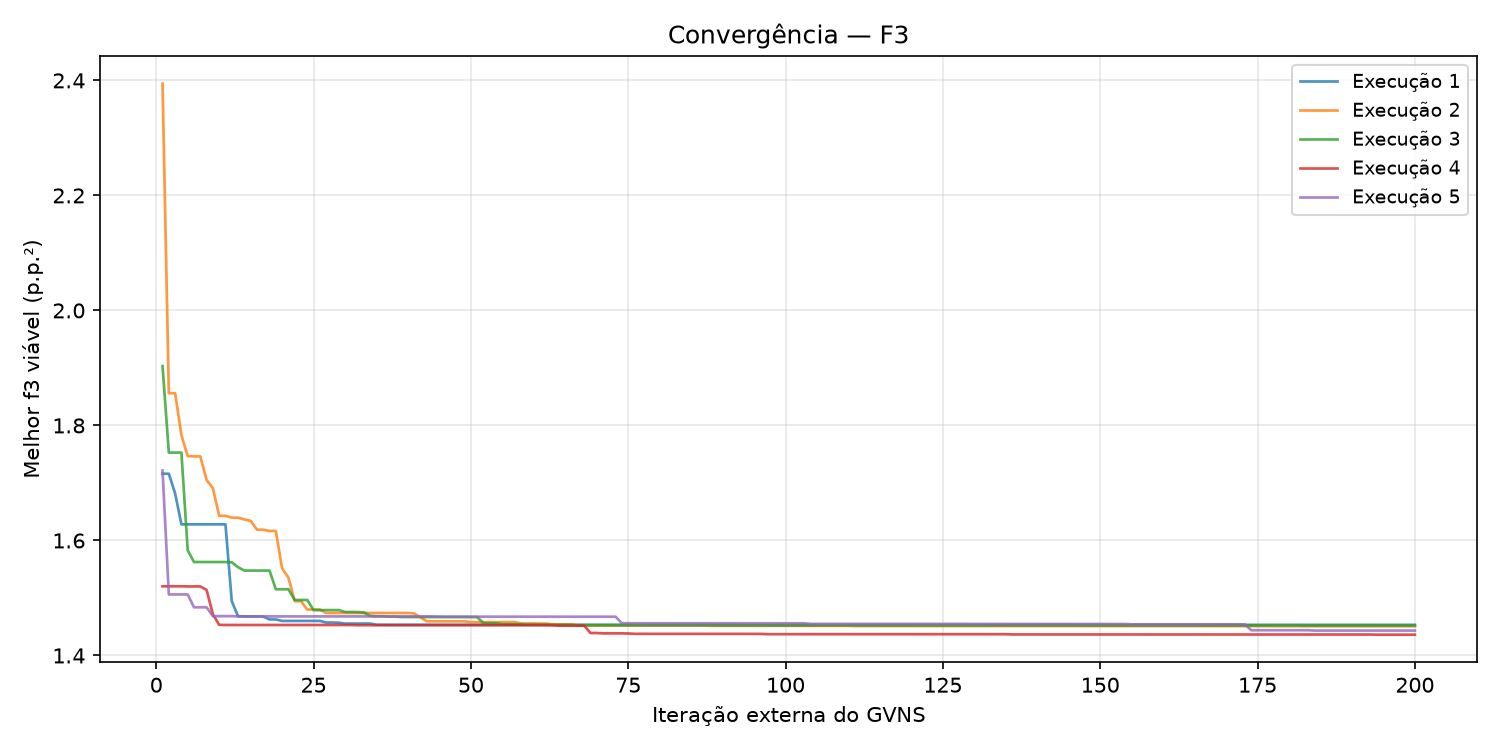
\includegraphics[width=0.88\textwidth]{results/tp1_corrigido/convergencia_f3.png}

\caption{Melhor valor viável observado de $f_3$ nas cinco execuções}

\label{fig:conv_f3}

\end{figure}

\subsection{Melhores composições e compromissos}

As barras mostram caminhões de 2 kt por minério em cada pilha; as alturas vão de 10 a 19 caminhões. As composições completas estão nos registros JSON.

\begin{figure}[H]\centering

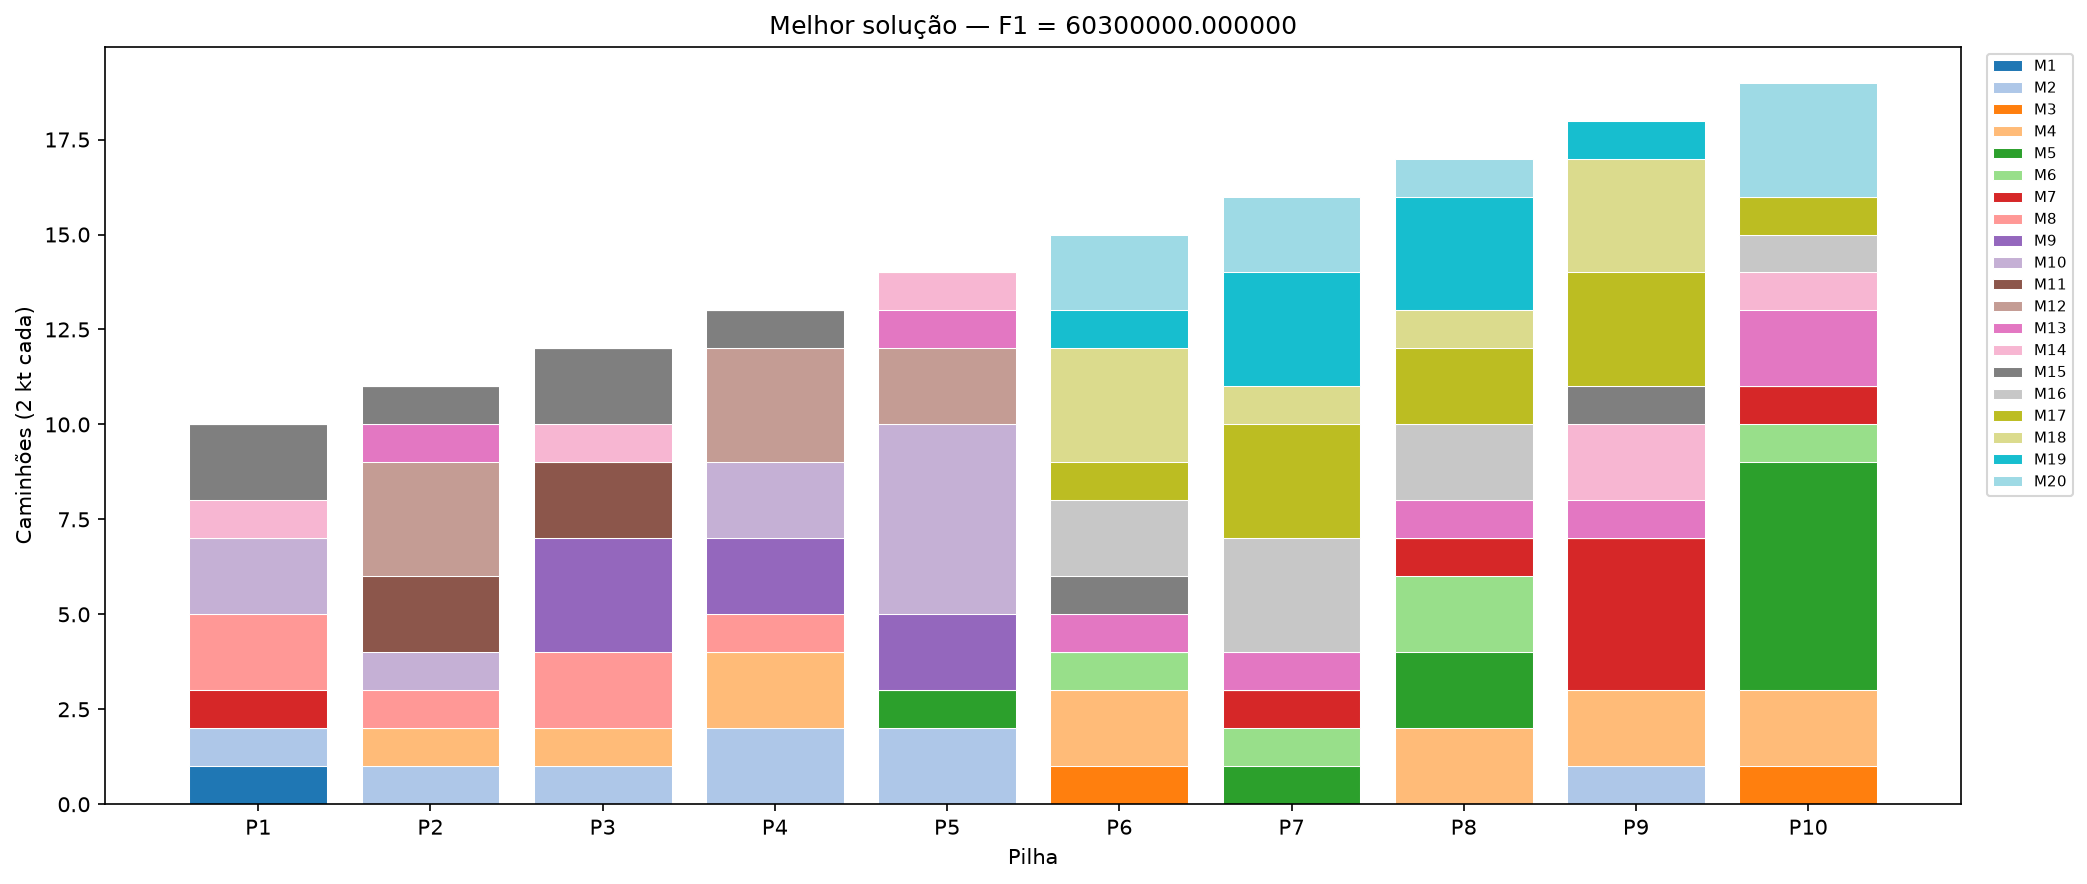
\includegraphics[width=\textwidth]{results/tp1_corrigido/melhor_solucao_f1.png}

\caption{Melhor composição para $f_1=\num{60300000}$ (seed 789)}

\label{fig:sol_f1}

\end{figure}

\begin{figure}[H]\centering

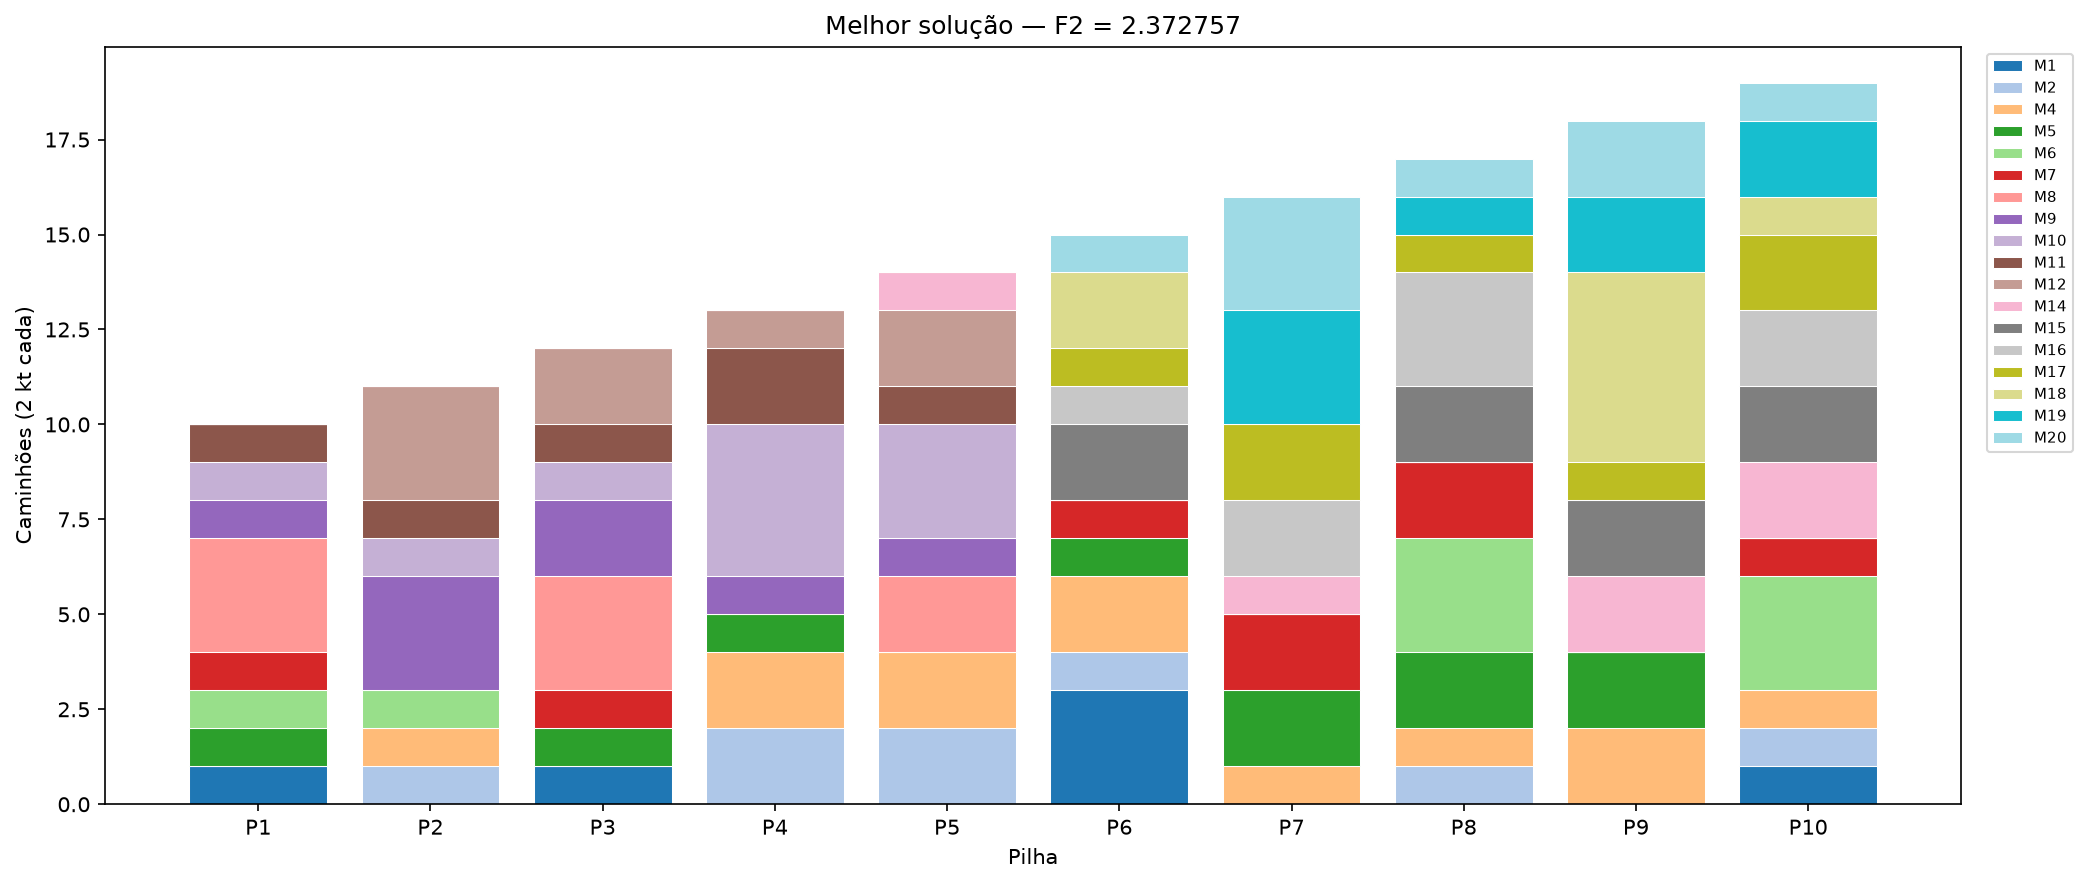
\includegraphics[width=\textwidth]{results/tp1_corrigido/melhor_solucao_f2.png}

\caption{Melhor composição para $f_2=\num{2.372757}$ (seed 456)}

\label{fig:sol_f2}

\end{figure}

\begin{figure}[H]\centering

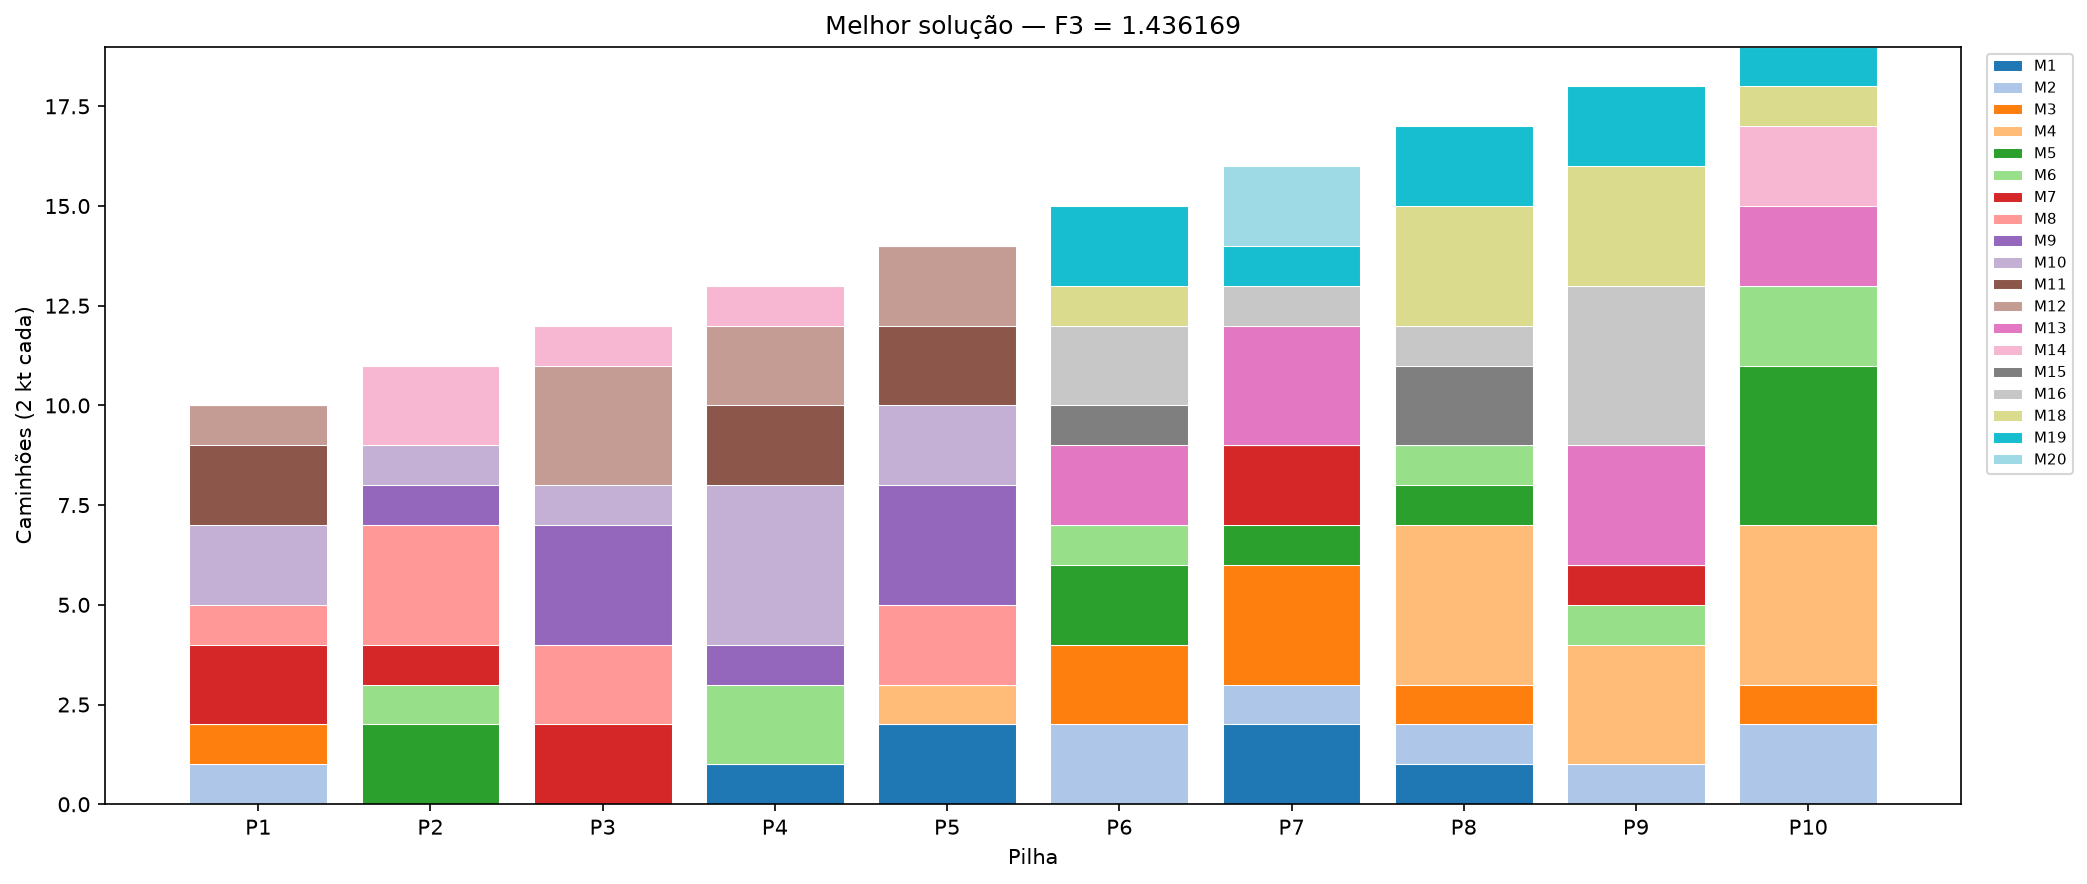
\includegraphics[width=\textwidth]{results/tp1_corrigido/melhor_solucao_f3.png}

\caption{Melhor composição para $f_3=\num{1.436169}$ (seed 789)}

\label{fig:sol_f3}

\end{figure}

\begin{table}[H]\centering\small

\caption{Matriz cruzada das melhores soluções mono-objetivo}

\begin{tabular}{lrrr}\toprule

Objetivo otimizado & $f_1$ (R\$) & $f_2$ (p.p.$^2$) & $f_3$ (p.p.$^2$) \\ \midrule

$f_1$ & \num{60300000} & \num{6.410508} & \num{5.995129} \\

$f_2$ & \num{63440000} & \num{2.372757} & \num{3.665272} \\

$f_3$ & \num{65740000} & \num{5.955709} & \num{1.436169} \\

\bottomrule\end{tabular}\end{table}

A matriz evidencia que os desempenhos devem ser comparados na mesma composição. O mínimo de cada coluna da tabela das cinco rodadas pertence a uma otimização independente; combinar esses três mínimos não define uma receita realizável. A matriz cruzada conserva os três valores de cada alternativa.

\subsection{Referências para a próxima etapa}

Os extremos abaixo são calculados sobre os 15 vetores finais viáveis, incluindo os valores de cada objetivo nas buscas dos outros dois. São referências empíricas, não provas de ideal, nadir ou ótimo global.

\begin{table}[H]\centering\small

\caption{Extremos empíricos para normalização na Entrega 2}

\begin{tabular}{lrr}\toprule Objetivo & Mínimo observado & Máximo observado \\ \midrule

$f_1$ & \num{60300000} & \num{65840000} \\

$f_2$ & \num{2.372757} & \num{6.705745} \\

$f_3$ & \num{1.436169} & \num{5.995129} \\

\bottomrule\end{tabular}\end{table}

Cada extremo aponta ao identificador da execução e ao hash do arquivo que contém sua composição em \texttt{referencias\_tp1.json}. A próxima etapa aplicará a mesma transformação min--max nos dois métodos. Novas soluções poderão extrapolar o intervalo empírico; os valores não devem ser truncados.

\subsection{Análise da revisão}

O acompanhamento separado pode melhorar o retorno sem alterar a trajetória estocástica por fitness: candidatos viáveis anteriormente descartados como incumbentes agora continuam disponíveis. Por isso, diferenças em relação ao log histórico não são tratadas como erro de reprodução. A disponibilidade das 15 composições permite conferir cada uma das alegações de viabilidade.

$f_1$: coeficiente de variação amostral de \num{0.2720}\%.

$f_2$: coeficiente de variação amostral de \num{0.0229}\%.

$f_3$: coeficiente de variação amostral de \num{0.5013}\%.

Com cinco sementes, essa comparação é descritiva e não comprova superioridade estatística, otimalidade ou cobertura do espaço de soluções.

\section{Conclusão}

As 15 soluções finais foram validadas individualmente e por auditoria independente. A base mono-objetivo corrigida, com registros e referências empíricas rastreáveis, está pronta para a etapa multiobjetivo.
